\section{场景及假设}
\label{sec:featurespy-setting}
本文提出 \sysnameF 通过在客户端 {\em 可信执行环境 (TEE)} 中通过 {\em 主动检测学习内容攻击} 来增强加密后重复数据删除,从而完全击败恶意客户端。

\paragraph*{Trusted execution.} 我们建立在 {\em Intel Software Guarded Extensions (SGX)} \cite{sgx} 上来实现 TEE,因为 SGX 得到了当今商品计算机的广泛支持。除了 SGX,我们的设计 (\S\ref{sec:featurespy-design}) 可以扩展到其他支持 TEE 的可信计算技术 \cite{amd-sev, pinto19}。

SGX 使用一组与安全相关的指令扩展 Intel CPU 以实现 TEE。它在硬件保护的内存区域(称为 {\em 安全区页面缓存 (EPC)})中分配一个 {\em 安全区},以便在具有机密性和完整性保证的情况下托管(in-enclave)内容。创建安全区后,SGX 提供 {\em 远程认证} 以通过远程实体(例如,云)对安全区进行身份验证,以及 {\em 安全密封} 在(经过身份验证的)enclave 和云端。此外,SGX 为安全区和未受保护的内存之间的交互提供了两个接口。程序可以通过 {\em 安全区调用 (ECalls)} 进入安全区执行安全区内部函数。在 ECall 中,它可以暂时退出安全区并通过 {\em 安全区外部调用 (OCalls)} 在不受保护的内存中调用不受信任的函数。



\paragraph*{部署场景。}图~\ref{fig:featurespy-model}展示了加密后重复数据删除的场景(\S\ref{subsec:featurespy-basics})。为了部署 \sysnameF,我们首先将安全区代码编译成共享对象 \cite{sgx},并将共享对象连同用于完整性验证的签名分发给每个客户端。云托管共享对象以验证每个客户端的安全区。具体来说,客户端初始化\sysnameF,通过加载共享对象创建对应的enclave,云端通过远程证明\cite{sgx}对每个enclave进行认证,以确保将正确的代码加载到enclave中。

在上传过程中,\sysnameF 处理明文块(由客户端生成),并为基于数据源的重复数据删除计算相应的密文块和指纹。未受损的客户端仅将不重复的密文块传输到云,而 \sysnameF 如果客户端被捕获以发起学习内容攻击,则会报告恶意客户端。

\begin{figure}
  \centering
  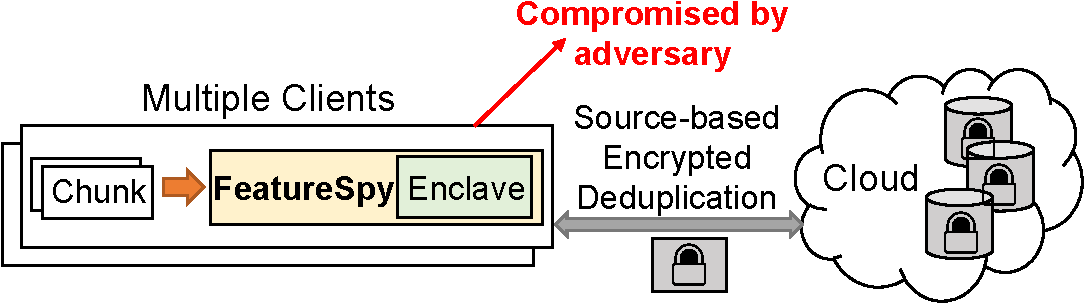
\includegraphics[width=\textwidth]{pic/featurespy/deployment.pdf}
  \vspace{-6pt}
  \caption{部署 \sysnameF.}
  \label{fig:featurespy-model}
  \vspace{-6pt}
\end{figure}

\paragraph*{威胁模型。} 我们的主要安全目标是增强加密后重复数据删除 (\S\ref{subsec:featurespy-basics}) 以防止 {\em 恶意} 客户端的安全性。与加密后重复数据删除 \cite{bellare13a} 一样,我们考虑了一个旨在从任何存储的密文块中窃听原始内容的受损云。此外,我们考虑一个恶意客户端,旨在学习其他未受损客户端的原始明文块。具体来说,恶意客户端可以访问其受损的明文块和密钥,并任意伪造新的明文块以发起学习内容攻击(\S\ref{subsec:featurespy-basics})。此外,它可以篡改未受保护的内存中的内容和操作,以逃避 \sysnameF 的捕获。

我们的威胁模型做出以下假设。
\begin{itemize}[leftmargin=*]
\item
  每个客户端与云之间的通信通道受 SSL/TLS 保护以防窃听。
\item
  SGX安全区是受信任和经过身份验证的(例如,在首次引导时通过远程证明),以便诚实地执行攻击检测以防止篡改。此外,与之前的作品 \cite{shinde20, ren21} 一样,SGX安全区只为加密密钥(即 \S\ref{sec:featurespy-implementation} 中的证明密钥)而不是所有安全区内的内容保留机密性;鉴于针对 SGX 的侧信道攻击,这一点很重要(例如,请参阅 \cite{fei21} 进行调查)。
\item
  恶意云可能会破坏外包数据以损害完整性。 \sysnameF 没有解决威胁,但它与 \textit{  (proof data prosession,PDP)} \cite{ateniese07} 和 \textit{  (proof of retrievability,PoR)} \cite{juels07} 兼容,以执行定期的完整性验证外包数据,以及容错存储,以从损坏 \cite{li15} 中恢复数据。
\end{itemize}